\documentclass[compress,color=usenames]{beamer}

\newcommand{\mytitlenbr}{1}
\newcommand{\mytitle}{Image Archive}

%\documentclass[compress,color=usenames,handout]{beamer}

%\usepackage{pgfpages}
%\pgfpagelayout{4 on 2}[a4paper,border shrink=5mm]

\usepackage{graphicx}
\usepackage{amsfonts,amssymb}
\usepackage{latexsym}
\usepackage{mdwtab}
\usepackage{xspace}
\usepackage{tikz}
\usetikzlibrary{shapes,snakes}
\usetikzlibrary{petri}

\DefineNamedColor{named}{Periwinkle}{cmyk}{0.57,0.55,0,0}
\DefineNamedColor{named}{Plum}{cmyk}{0.50,1,0,0}
\DefineNamedColor{named}{Red}{cmyk}{0,1,1,0}

\newcommand{\mH}[1]{\textcolor{Plum}{#1}}
\newcommand{\mT}[1]{\textcolor{Periwinkle}{#1}}

\newcommand{\tup}[1]{\langle #1 \rangle}

\newcommand{\dd}{{:}}
\newcommand{\I}{\mathcal{I}}
\newcommand{\csetsc}[2]{\{#1 \mid #2\}}
\newcommand{\cset}[1]{\{#1\}}

\newcommand{\CON}{\textsf{CON}\xspace}
\newcommand{\ROL}{\textsf{ROL}\xspace}
\newcommand{\IND}{\textsf{IND}\xspace}
\newcommand{\PROP}{\textsf{PROP}\xspace}
\newcommand{\lang}{\mathcal{L}\xspace}


\newcommand{\mytt}[1]{\textsf{\scriptsize{#1}}}
\newcommand{\mytts}[1]{\textsf{\scriptsize{#1}}}

%\usefonttheme{serif}

\mode<presentation>
 {
 \usetheme{lined}
 }

\setbeamertemplate{navigation symbols}{}


\newcommand{\F}{\mathop{\mathsf{F}\vphantom{a}}\nolimits}
\newcommand{\G}{\mathop{\mathsf{G}\vphantom{a}}\nolimits}
\newcommand{\X}{\mathop{\mathsf{X}\vphantom{a}}\nolimits}

\newcommand{\Blue}[1]{\textcolor{blue}{#1}}
\newcommand{\Red}[1]{\textcolor{red}{#1}}
\newcommand{\Green}[1]{\textcolor{PineGreen}{#1}}


\title[GLN y Aplicaciones]{\Huge Generaci\'on de Lenguaje Natural y Aplicaciones}
%\mH{Lecture \#\mytitlenbr:} \mytitle}

\author[Areces \& Benotti]{
 Carlos Areces y Luciana Benotti\\[1ex]
\normalsize \url{{carlos.areces, luciana.benotti}@gmail.com}}

\institute[INRIA / UNC]{
INRIA Nancy Grand Est, Nancy, France\\
Universidad Nacional de C\'ordoba, C\'ordoba, Argentina}

\date{ELiC 2010 - Buenos Aires - Argentina}

\begin{document}


\beamerdefaultoverlayspecification{}


\begin{frame}[plain]
 \titlepage
\end{frame}

\begin{frame}
%\frametitle{What This Tutorial is About}
\frametitle{De que se Trata este Curso?}

\begin{itemize}
\item Vamos a hablar de la Generaci\'on Autom\'atica de Lenguaje Natural
\item Es decir, el dise\~no e implementaci\'on de sistemas que 
\begin{itemize}
\item producen texto comprensible en lenguaje natural (e.g., Castellano, 
Ingl\'es, etc.)
\item a partir de una representaci\'on no ling\"u\'istica de informaci\'on
\item usando conocimiento acerca del lenguaje y del dominio de aplicaci\'on.
\end{itemize}

\end{itemize}

%\label{f0}
%\begin{itemize}
%\item { {The design and construction of systems which}}
%\begin{itemize}
%\item produce understandable texts in English or other human languages ...
%\item from some underlying non-linguistic representation of information 
%\item using knowledge about language and the application domain.
%\end{itemize}
%\end{itemize}

\end{frame}

\begin{frame}
\frametitle{Objetivos del Curso}

\begin{itemize}
\item Dar un panorama amplio del \'area y de lo que es posible hacer hoy en d\'ia.
\item Introducir en detalle algunas de las t\'ecnicas (algunas b\'asicas y otras 
m\'as avanzadas) del \'area. 
\item Discutir algunos temas que son importantes para la aplicaci\'on de 
t\'ecnicas de GLN en proyectos concretos.
\end{itemize}
\end{frame}

\begin{frame}
\frametitle{Estructura del Curso}

\begin{columns}
\column{1.1\textwidth}
\begin{itemize}
\item \mH{Primera Parte}: Carlos Areces
\begin{itemize}
\item \mH{Lunes:} El Problema de Generaci\'on de Lenguaje Natural. Algunos systemas de GNL.  GNL Pipeline. Representaci\'on de Informaci\'on e Inferencia para GLN. Evaluaci\'on de Sistemas de GLN.\pause

\item \mH{Martes:} Tree Adjoining Grammars (TAG). Interface Sint\'actica-Sem\'antica.
Realizaci\'on. Realizaci\'on via via Charts. \pause

\item \mH{Mi\'ercoles:} Algoritmos de Generaci\'on de Expresiones Referenciales. Informaci\'on Proposicional vs.\ Informaci\'on Relacional. Optimizaci\'on de Algoritmos. Evaluaci\'on.\pause
\end{itemize}

\item \mH{Segunda Parte}: Luciana Benotti

\begin{itemize}
\item \mH{Jueves:} Entornos Virtuales (e.g., Second Life) y Aplicaciones (e.g., Tutoring) para Sistemas de GNL. Inferencia Orientada a Metas. Algoritmos de Planning y su uso en Entornos Virtuales.\pause

\item \mH{Viernes:} Generaci\'on de Referencias en un Entorno Virtual. Estrategias de Referencia. Supervisi\'on de la Interpretaci\'on. Evaluaci\'on.
\end{itemize}
\end{itemize}
\end{columns}
\end{frame}

\begin{frame}
\frametitle{Lo que Veremos Hoy}

\begin{itemize}
\item  Introducci\'on a GLN 
\item  Un Caso de Estudio
\item  Las Tareas b\'asicas de GLN
\item  NLG en Ambientes Multimedia y Multimodales
\item Evaluaci\'on de Systemas de GLN
\end{itemize}
\end{frame}


\begin{frame}
\frametitle{Lo que Veremos Hoy}

\begin{itemize}
\item  Introducci\'on a GLN 
\begin{tabular}{|l}
 {\small Que es GLN?}\\
 {\small Ejemplos}\\
 {\small Aplicaciones t\'ipicas de GLN}\\
 {\small Cuando es apropiado usar GLN?}\\
 {\small La Arquitectura de un systema de NLG}
\end{tabular}

\item  Un Caso de Estudio
\item  Las Tareas b\'asicas de GLN
\item  NLG en Ambientes Multimedia y Multimodales
\item Evaluaci\'on de Systemas de GLN
\end{itemize}
\end{frame}

\begin{frame}
\frametitle{Qu\'e es GLN?}

\begin{itemize}
\item { {Natural language generation is the process of deliberately constructing a natural language text in order to meet specified communicative goals.}}\\

\hfill [McDonald 1992]
\end{itemize}


\end{frame}

\begin{frame}
\frametitle{Qu\'e es GLN?}

\begin{itemize}
\item  \mH{Objetivo: }

\begin{itemize}
\item software que produce texto entendible y adecuado en lenguaje natural (e.g., Ingl\'es).
\end{itemize}

\item  \mH{Input: }
\begin{itemize}
\item Informaci\'on no ling\"u\'istica (e.g., una base de datos)
\end{itemize}

\item  \mH{Output: }
\begin{itemize}
\item documentoss, reportes, explicaciones, mensajes de ayuda, etc.
\end{itemize}

\item \mH{Informaci\'on requerida: }
\begin{itemize}
\item Conocimiento dle lenguaje y del dominio de aplicaci\'on
\end{itemize}
\end{itemize}

\end{frame}

\begin{frame}
\frametitle{Generaci\'on vs. Interpretaci\'on}

\begin{center}
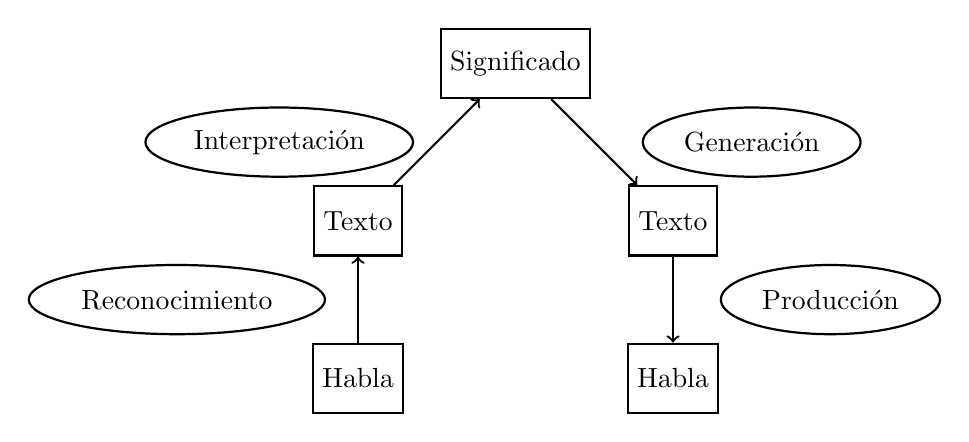
\begin{tikzpicture}[style=thick]

\node (n1) at (0,0) [rectangle, draw, minimum size=25pt]{Significado};

\node (l1) at (-3,-1) [ellipse, draw, minimum size=25pt]{Interpretaci\'on};
\node (l2) at (3,-1) [ellipse, draw, minimum size=25pt]{Generaci\'on};

\node (n2) at (-2,-2) [rectangle, draw, minimum size=25pt]{Texto};
\node (n3) at (2,-2) [rectangle, draw, minimum size=25pt]{Texto};

\node (l1) at (-4.3,-3) [ellipse, draw, minimum size=25pt]{Reconocimiento};
\node (l2) at (4,-3) [ellipse, draw, minimum size=25pt]{Producci\'on};

\node (n4) at (-2,-4) [rectangle, draw, minimum size=25pt]{Habla};
\node (n5) at (2,-4) [rectangle, draw, minimum size=25pt]{Habla};

\draw [->] (n2) to (n1);
\draw [->] (n1) to (n3);

\draw [->] (n4) to (n2);
\draw [->] (n3) to (n5);

\end{tikzpicture}
\end{center}

%\begin{center}
%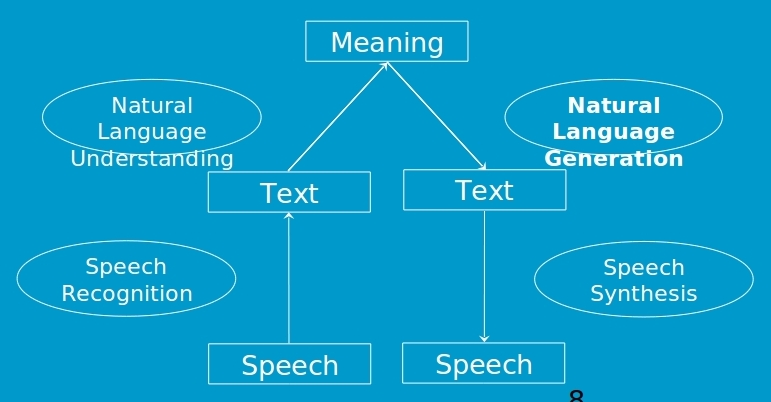
\includegraphics[scale=.3]{pics/pic1.jpg}
%\end{center}
\end{frame}

\begin{frame}
\frametitle{Sistema Ejemplo \#1: FoG}

\begin{itemize}
\item \mH{Funci\'on: }
\begin{itemize}
\item Producir reportes clim\'aticos en formato texto  en Ingl\'es y en Franc\'es.
\end{itemize}
\item \mH{Input: }
\begin{itemize}
\item Im\'agen gr\'afica clim\'atica con informaci\'on num\'erica
\end{itemize}
\item \mH{Usuario: }
\begin{itemize}
\item Environment Canada (Servicio Clim\'atico Canadiense)
\end{itemize}
\item \mH{Status: }
\begin{itemize}
\item Funcionando desde 1992
\end{itemize}
\end{itemize}
\end{frame}

\begin{frame}
\frametitle{FoG: Input}

\begin{center}
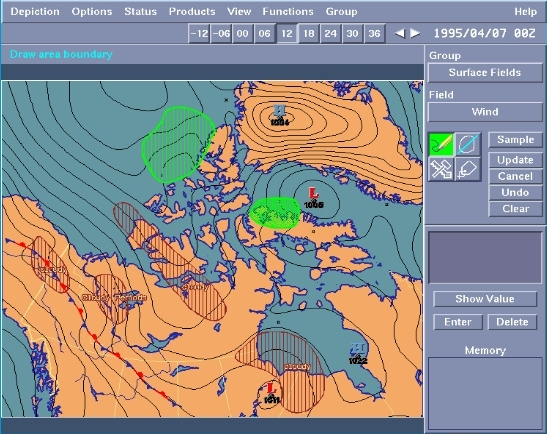
\includegraphics[scale=.4]{pics/pic2.jpg}
\end{center}

\end{frame}

\begin{frame}
\frametitle{FoG: Output}

\begin{center}
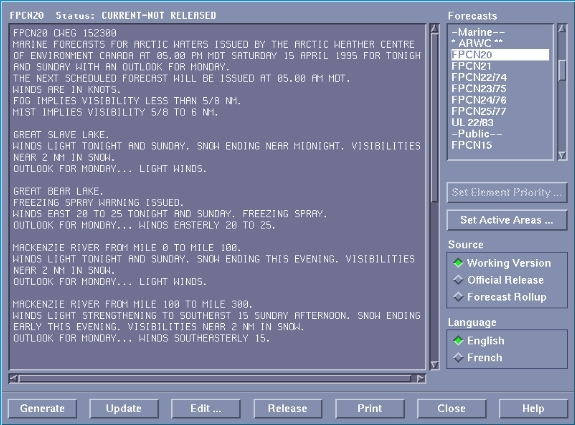
\includegraphics[scale=.4]{pics/pic3.jpg}
\end{center}

\end{frame}

\begin{frame}
\frametitle{Sistema Ejemplo \#2: PlanDoc}

\begin{itemize}
\item \mH{Funci\'on: }
\begin{itemize}
\item Producir un reporte describiendo las opciones de simulaci\'on que un ingeniero ya ha explorado
\end{itemize}
\item \mH{Input: }
\begin{itemize}
\item Un archivo de log de simulaciones
\end{itemize}
\item \mH{Usuario: }
\begin{itemize}
\item Southwestern Bell
\end{itemize}
\item \mH{Status: }
\begin{itemize}
\item Funcionando desde 1996
\end{itemize}
\end{itemize}

\end{frame}

\begin{frame}[fragile]
\frametitle{PlanDoc: Input}

\begin{verbatim}
  RUNID fiberall FIBER 6/19/93 act yes
  FA 1301 2 1995
  FA 1201 2 1995
  FA 1401 2 1995
  FA 1501 2 1995
  ANF co 1103 2 1995 48
  ANF 1201 1301 2 1995 24
  ANF 1401 1501 2 1995 24
  END. 856.0 670.2
\end{verbatim}

\end{frame}

\begin{frame}
\frametitle{PlanDoc: Output}

This saved fiber refinement includes all DLC changes in Run-ID ALLDLC. RUN-ID FIBERALL demanded that PLAN activate fiber for CSAs 1201, 1301, 1401 and 1501 in 1995 Q2. It requested the placement of a 48-fiber cable from the CO to section 1103 and the placement of 24-fiber cables from section 1201 to section 1301 and from section 1401 to section 1501 in the second quarter of 1995. For this refinement, the resulting 20 year route PWE was \$856.00K, a \$64.11K savings over the BASE plan and the resulting 5 year IFC was \$670.20K, a \$60.55K savings over the BASE plan.
\end{frame}

\begin{frame}
\frametitle{Sistema Ejemplo \#3: STOP}

\begin{itemize}
\item \mH{Function: }
\begin{itemize}
\item Producir un folleto presonalizado para ayudar a dejar de fumar 
\end{itemize}
\item \mH{Input: }
\begin{itemize}
\item Questionario sobre historia, creencias, actitudes, etc.\ sobre el cigarrillo
\end{itemize}
\item \mH{Usuario: }
\begin{itemize}
\item NHS (British Health Service)
\end{itemize}
\item \mH{Status: }
\begin{itemize}
\item Utilizado por varios a\~nos
\end{itemize}
\end{itemize}

\end{frame}

\begin{frame}
\frametitle{STOP: Input}

\begin{center}
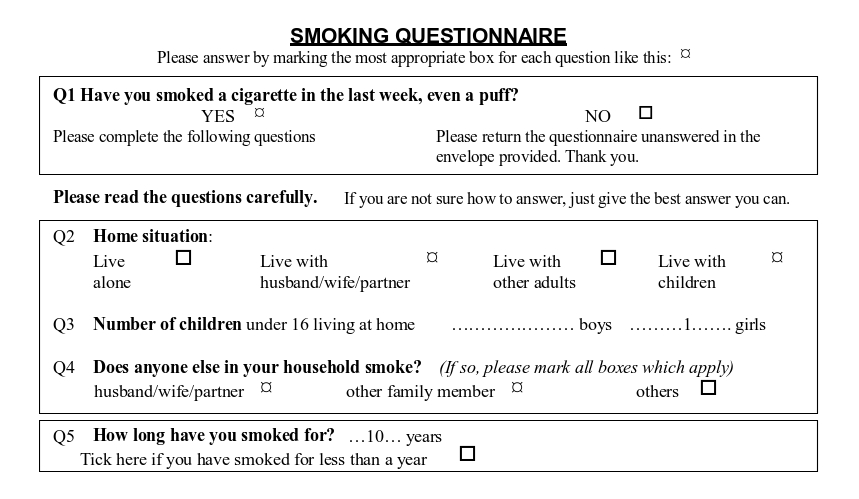
\includegraphics[scale=.4]{pics/pic4.jpg}
\end{center}

\end{frame}

\begin{frame}
\frametitle{STOP: Output}

Dear Ms Cameron\\ \ \\

 { {Thank you for taking the trouble to return the smoking questionnaire that we sent you. It appears from your answers that although you're not planning to stop smoking in the near future, you would like to stop if it was easy. You think it would be difficult to stop because \textit{smoking helps you cope with stress, it is something to do when you are bored, and smoking stops you putting on weight}. However, you have reasons to be confident of success if you did try to stop, and there are ways of coping with the difficulties. }}

\end{frame}

\begin{frame}
\frametitle{Sistema Ejemplo \#4: TEMSIS}

\begin{itemize}
\item \mH{Funci\'on: }
\begin{itemize}
\item Sumarizaci\'on de informaci\'on sobre contaminaci\'on
\end{itemize}
\item \mH{Input: }
\begin{itemize}
\item Datos ambientales + una pregunta espec\'ifica
\end{itemize}
\item \mH{Usuario: }
\begin{itemize}
\item Agencias ambientales en Francia y Alemania
\end{itemize}
\item \mH{Status: }
\begin{itemize}
\item Prototipos fueron instalados en la region Saar/Alsacia (borde entre Alemania y Francia). 
\end{itemize}
\end{itemize}

\end{frame}

\begin{frame}[fragile]
\frametitle{TEMSIS: Input Query}

\begin{verbatim}
((LANGUAGE FRENCH)
  (GRENZWERTLAND GERMANY)
  (BESTAETIGE-MS T)
  (BESTAETIGE-SS T) 
  (MESSSTATION \"Voelklingen City\"
  (DB-ID \"#2083\"
  (SCHADSTOFF \"#19\"
  (ART MAXIMUM)
  (ZEIT ((JAHR 1998)
         (MONAT 7)
         (TAG 21))))
\end{verbatim}

\end{frame}

\begin{frame}
\frametitle{TEMSIS: Output Summary}

\begin{itemize}
\item \mH{Franc\'es:}

Le 21/7/1998 \`a la station de mesure de V\"olklingen-City, la valeur moyenne maximale d'une demi-heure (Halbstundenmittelwert) pour l'ozone atteignait 104.0 $\mu$g/m${}^3$. Par cons\'equent, selon le decret MIK (MIK-Verordnung), la valeur limite autoris\'ee de 120 $\mu$g/m${}^3$ n'a pas \'et\'e d\'epass\'e.

\item \mH{Alem\'an:}

Der h\"ochste Halbstundenmittelwert f\"ur Ozon an der Me{\ss}station V\"olklingen-City erreichte 
am 21.7.1998 104.0 $\mu$g/m${}^3$, womit der gesetzlich zul\"assige Grenzwert nach MIK-Verordnung von 
120 $\mu$g/m${}^3$ nicht \"uberschritten wurde.
\end{itemize}

\end{frame}

\begin{frame}
\frametitle{Tipos de Aplicaciones de NLG}

\begin{itemize}
\item \mH{Producci\'on autom\'atica de documentos}
\begin{itemize}
\item reportes clim\'aticos, reporte de simulaciones, cartas, \ldots
\end{itemize}
\item \mH{Presentaci\'on de informaci\'on al p\'ublico en forma entendible}
\begin{itemize}
\item imformes m\'edicos, sistemas expertos de inferencia, \ldots
\end{itemize}
\item \mH{Ense\~nanza}
\begin{itemize}
\item educaci\'on a distancia
\end{itemize}
\item \mH{Entretenimiento/Arte}
\begin{itemize}
\item bromas (?), historias (??), poes\'ia (???)
\end{itemize}
\end{itemize}

\end{frame}

\begin{frame}
\frametitle{El Rol de la Computadora}

 Dos posibilidades
\begin{itemize}
\item \#1 El sisema produce un documento autom\'aticamente (sin ayuda humana) 

 reportes clim\'aticos, reportes de simulaciones, cartas a pacientes,
 res\'umenes de datos estad\'isticos, explicaciones en sistemas expertos.

\item \#2 El sistema ayuda a un autor humano a crear un documento:

 reportes clim\'aticos, reportes de simulaciones, cartas a pacientes
 pedidos de patentes, documentos t\'ecnicos (manuales), pedidos de empleo
\end{itemize}

\end{frame}

\begin{frame}
\frametitle{En qu\'e casos son las t\'ecnicas de GLN Adecuadas?}

Opciones a Considerar:

\begin{itemize}
\item { {Texto vs.\ Gr\'aficos}}
\begin{itemize}
\item Qu\'e medio es mejor?
\end{itemize}
\item { {Generaci\'on Autom\'atica vs. Autor\'ia Humana}}
\begin{itemize}
\item Son los datos necesarios accesibles? 
\item Vale la pena (e.g., econ\'omicamente)?
\end{itemize}
\item { {GLN vs. Concatenaci\'on de strings}}
\begin{itemize}
\item Cu\'anta variaci\'on hay en el texto?
\item Que impacto tiene la calidad gramatical del texto? 
\end{itemize}
\end{itemize}

\end{frame}

\begin{frame}
\frametitle{Calidad Gramatical}

\begin{itemize}
\item La generaci\'on de texto ling\"u\'isticamente bien formado requiere la verificaci\'on de constraints
\begin{itemize}
\item ortogr\'aficos, morfol\'ogicos, sint\'acticos
\item referencia, elecci\'on de palabras, pragm\'aticas
\end{itemize}
\item Estos constraints se verifican autom\'aticamente por un sistema de GLN
\begin{itemize}
\item en forma autom\'atica, el 100\% de los casos
\end{itemize}
\item Los desarrolladores de sistemas basados en concatenaci\'on de strings tienen que verificar
 el cumplimiento de estos strings manualmente y v\'ia testing
\begin{itemize}
\item Muy trabajoso
\item Dif\'icil de garantizar exactitud del 100\%
\end{itemize}
\end{itemize}

\end{frame}

\begin{frame}
\frametitle{Ejemplo: Syntaxis, agregaci\'on}

\label{f48}
\begin{itemize}
\item { {Output de sistemas de IA Medical existentes:}}

\begin{quote}
 The primary measure you have chosen, CXR shadowing, should be justified in comparison to TLC and walking distance as my data reveals they are better overall. Here are the specific comparisons:
\medskip

 TLC has a lower patient cost TLC is more tightly distributed TLC is more objective walking distance has a lower patient cost
\end{quote}
\end{itemize}

\end{frame}

\begin{frame}
\frametitle{Ejemplo: Pragm\'atica}

\label{f50}
\begin{itemize}
\item Output de un sistema que da versiones en ingl\'es de consultas a una base de datos:

\begin{quote} 
The number of households such that there is at least 1 order with dollar amount greater 
than or equal to \$100.\pause
\end{quote}

\begin{itemize}

\item Se interpreta como ``number of households which have placed an order 
\mbox{$>=$} \$100'' \pause
\item La consulta inicial era el n\'umero total de casas en la base de datos, si habia alguna 
orden en la base de datos (de cualquier casa) por mas de \$100
\end{itemize}
\end{itemize}

\end{frame}

\begin{frame}
\frametitle{La Arquitectura de un Systema de GLN}

]\begin{itemize}
\item { {Las tareas b\'asicas en un sistema de GLN}}
\item Arquitectura de Pipeline 
\item Alternative Architectures
\end{itemize}

\end{frame}

\begin{frame}
\frametitle{Las Tareas B\'asicas en un sistema de GLN}

\label{f54}
\begin{enumerate}
\item { { Determinaci\'on de Contenido (Content determination)}}
\item { { Estructuraci\'on del Documento (Document structuring)}}
\item { { Agregaci\'on (Aggregation)}}
\item { { Lexicalizaci\'on (Lexicalisation)}}
\item { { Generaci\'on de Expresiones Referenciales (Referring expression generation)}}
\item { { Realizaci\'on Ling\"u\'istica (Linguistic realisation)}}
\item { { Realizaci\'on de Estructura (Structure realisation}}
\end{enumerate}

\end{frame}

\begin{frame}
\frametitle{Las Tareas B\'asicas en un sistema de GLN}

\begin{center}
\begin{tabular}{|l|c|}  \hline
Content Determination & Document \\
Document Structuring &  planning\\ \hline
Aggregation &  Micro-\\
Lexicalisation & planning\\
Referring Expression Generation & \\ \hline
Linguistic Realisation & Surface\\
Structure Realisation & realization\\ \hline
\end{tabular}
\end{center}

\end{frame}

\begin{frame}
\frametitle{Una Arquitectura Pipeline}

\begin{center}
Document\\
planning\\
$\downarrow$\\
Document plan\\
$\downarrow$\\
Microplanning\\
$\downarrow$\\
Text Specificacion\\
$\downarrow$\\
Surface\\
Realization
\end{center}

\end{frame}

\begin{frame}
\frametitle{Otras Arquitecturas}

\label{f60}
\begin{itemize}
\item { {\#1: Variaciones de la arquitectura ``standard'':}}
\begin{itemize}
\item { {Alterar el orden de las tareas}}
\item { {Permitir feedback entre las distintas etapas}}
\end{itemize}
\item { {\#2: Un sistema integrado donde todas las tareas se combinan:}}
\begin{itemize}
\item { {representar todas las tareas en forma uniforme: e.g.\ como constraints, axiomas, operadores de planning, \ldots}}
\item { {alimentar estas especificaciones a un  constraint-solver, demostrador de teoremas, \ldots}}
\end{itemize}
\end{itemize}
\end{frame}

\begin{frame}
\frametitle{Temas de Investigaci\'on}

\label{f62}
\begin{itemize}
\item { {Cu\'ando es texto la mejor forma de cominicarse con el usuario??}}
\item { {Cu\'ando es GLN mejor que concatenaci\'on de strings?}}
\item { {Existe alguna arquitectura que combine la elegancia te\'orica y la flexibilidad de un sistema integrado, con la simplicidad de una arquitectura pipeline?}}
\item { {Como debemos representar planes de documento y expecificaciones de texto?}}
\end{itemize}

\end{frame}

\begin{frame}
\frametitle{Overview}

\label{f64}
\begin{itemize}
\item { {1 An Introduction to NLG}}
\item { {2 Requirements Analysis and a Case Study}}
\item { {3 The Component Tasks in NLG}}
\item { {4 NLG in Multimedia and Multimodal Systems}}
\item { {5 Conclusions and Pointers}}
\end{itemize}

\end{frame}

\begin{frame}
\frametitle{A Case Study in Applied NLG}

\begin{itemize}
\item { {Each month an institutional newsletter publishes a summary of the month's weather}}
\item { {The summaries are based on automatically collected meteorological data}}
\item { {The person who writes these summaries will no longer be able to}}
\item { {The institution wants to continue publishing the reports and so is interested in using NLG techniques to do so}}
\end{itemize}

\end{frame}

\begin{frame}
\frametitle{A Weather Summary}

\begin{center}
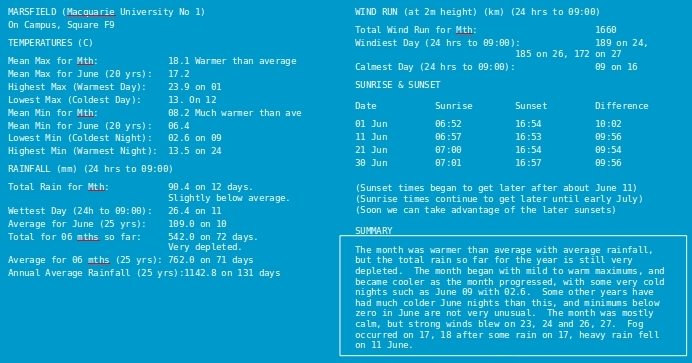
\includegraphics[scale=.47]{pics/pic5.jpg}
\end{center}

\end{frame}


\begin{frame}
\frametitle{Output: A Weather Summary}

\label{f70}
\begin{itemize}
\item { {The month was warmer than average with average rainfall, but the total rain so far for the year is still very depleted. The month began with mild to warm maximums, and became cooler as the month progressed, with some very cold nights such as June 09 with 02.6. Some other years have had much colder June nights than this, and minimums below zero in June are not very unusual. The month was mostly calm, but strong winds blew on 23, 24 and 26, 27. Fog occurred on 17, 18 after some rain on 17, heavy rain fell on 11 June.}}
\end{itemize}

\end{frame}

\begin{frame}[fragile]
\frametitle{The Input Data}

\begin{itemize}
\item { {A set of 16 data elements collected automatically every 15 minutes: air pressure, temperature, wind speed, rainfall }}
\item { {Preprocessed to construct DailyWeatherRecords:}}

\begin{verbatim}
((type dailyweatherrecord)
   (date ((day ...)
          (month ...)
          (year ...)))
 (temperature ((minimum ((unit degrees-centigrade)
                         (number ...)))
               (maximum ((unit degrees-centrigrade)
                         (number ...)))))
 (rainfall ((unit millimetres)
            (number ...))))
\end{verbatim}

\end{itemize}
\end{frame}

\begin{frame}
\frametitle{Other Available Data}

\label{f74}
\begin{itemize}
\item { {Historical Data: Average temperature and rainfall figures for each month in the Period of Record (1971 to present)}}
\item { {Historical Averages: Average values for temperature and rainfall for the twelve months of the year over the period of record}}
\end{itemize}

\end{frame}

\begin{frame}
\frametitle{Requirements Analysis}

\label{f76}
\begin{itemize}
\item { {The developer needs to:}}
\item { {understand the client\^as needs}}
\item { {propose a functionality which addresses these needs}}
\end{itemize}

\end{frame}

\begin{frame}
\frametitle{Corpus-Based Requirements Analysis}

\label{f78}
\begin{itemize}
\item { {A corpus:}}
\item { {consists of examples of output texts and corresponding input data}}
\item { {specifies \^aby example\^a the functionality of the proposed NLG system}}
\item { {is a very useful resource for design as well as requirements analysis}}
\end{itemize}

\end{frame}

\begin{frame}
\frametitle{Corpus-Based Requirements Analysis}

\label{f80}
\begin{itemize}
\item { {Four steps:}}
\item { {assemble an initial corpus of (human-authored) output texts and associated input data}}
\item { {analyse the information content of the corpus texts in terms of the input data}}
\item { {develop a target text corpus}}
\item { {create a formal functional specification}}
\end{itemize}

\end{frame}

\begin{frame}
\frametitle{Step 1: Creating an Initial Corpus}

\label{f82}
\begin{itemize}
\item { {Collect a corpus of input data and associated (human-authored) output texts}}
\item { {One source is archived examples of human-authored texts}}
\item { {If no human-authored examples of the required texts exist, ask domain experts to produce examples}}
\item { {The corpus should cover the full range of texts expected to be produced by the NLG system}}
\end{itemize}

\end{frame}

\begin{frame}
\frametitle{Initial Text (April 1995)}

\label{f84}
\begin{itemize}
\item { {SUMMARY}}
\item { {The month was rather dry with only three days of rain in the middle of the month. The total for the year so far is very depleted again, after almost catching up during March. Mars Creek dried up again on 30th April at the waterfall, but resumed on 1st May after light rain. This is the fourth time it dried up this year.}}
\end{itemize}

\end{frame}

\begin{frame}
\frametitle{Step 2: Analyzing the Content of the Texts}

\label{f86}
\begin{itemize}
\item { {Goal: }}
\begin{itemize}
\item to determine where the information present in the texts comes from, and the extent to which the proposed NLG system will have to manipulate this information
\end{itemize}
\item { {Result: }}
\begin{itemize}
\item a detailed understanding of the correspondences between the available input data and the output texts in the initial corpus
\end{itemize}
\end{itemize}


\end{frame}

\begin{frame}
\frametitle{Information Types in Text}

\label{f88}
\begin{itemize}
\item { {Unchanging text}}
\item { {Directly-available data}}
\item { {Computable data}}
\item { {Unavailable data}}
\end{itemize}

\end{frame}

\begin{frame}
\frametitle{Unchanging Text}

\mH{SUMMARY}

{ {The month was rather dry with only three days of rain in the middle of the month. The total for the year so far is very depleted again, after almost catching up during March. Mars Creek dried up again on 30th April at the waterfall, but resumed on 1st May after light rain. This is the fourth time it dried up this year.}}

\end{frame}

\begin{frame}
\frametitle{Directly Available Data}

SUMMARY

\mH{The month was rather dry with only three days of rain in the middle of the month}. The total for the year so far is very depleted again, after almost catching up during March. Mars Creek dried up again on 30th April at the waterfall, but resumed on 1st May after light rain. This is the fourth time it dried up this year.

\end{frame}

\begin{frame}
\frametitle{Computable Data}

SUMMARY

The month was rather dry with only three days of rain in the middle of the month. \mH{The total for the year so far is very depleted again, after almost catching up during March}. Mars Creek dried up again on 30th April at the waterfall, but resumed on 1st May after light rain. This is the fourth time it dried up this year.

\end{frame}

\begin{frame}
\frametitle{Unavailable Data}

SUMMARY

The month was rather dry with only three days of rain in the middle of the month. The total for the year so far is very depleted again, after almost catching up during March. \mH{Mars Creek dried up again on 30th April at the waterfall, but resumed on 1st May after light rain. This is the fourth time it dried up this year.}

\end{frame}


\begin{frame}
\frametitle{Solving the Problem of Unavailable Data}

\begin{itemize}
\item { {More information can be made available to the system: this may be expensive}}
    \begin{itemize}
        \item add sensors to Mars Creek?
    \end{itemize}
\item { {If the system is an authoring-aid, a human author can add this information}}
    \begin{itemize}
    \item system produces the first two sentences, the human adds the second two
    \end{itemize}
\item { {The target corpus can be revised to eliminate clauses that convey this information}}
    \begin{itemize}
    \item only produce the first two sentences
    \end{itemize}
\end{itemize}

\end{frame}

\begin{frame}
\frametitle{Step 3: Building theTarget Text Corpus}

\begin{itemize}
\item { {Mandatory changes:}}
\item { {eliminate unavailable data}}
\item { {specify what text portions will be human-authored}}
\item { {Optional changes:}}
\item { {simplify the text to make it easier to generate }}
\item { {improve human-authored texts}}
\item { {enforce consistency between human authors}}
\end{itemize}

\end{frame}

\begin{frame}
\frametitle{Target Text}

\begin{itemize}
\item { {The month was rather dry with only three days of rain in the middle of the month. The total for the year so far is very depleted again.}}
\end{itemize}

\end{frame}

\begin{frame}
\frametitle{Step 4: Functional Specification}

\label{f104}
\begin{itemize}
\item { {Based on an agreed target text corpus}}
\item { {Explicitly states role of human authoring, if present at all}}
\item { {Explicitly states structure and range of inputs to be used}}
\end{itemize}

\end{frame}

\begin{frame}
\frametitle{Initial Text \#2}

\label{f106}
\begin{itemize}
\item { {The month was our driest and warmest August in our 24 year record, and our first 'rainless' month. The 26th August was our warmest August day in our record with 30.1, and our first 'hot' August day (30). The month forms part of our longest dry spell 47 days from 18 July to 02 September 1995. Rainfall so far is the same as at the end of July but now is very deficient.}}
\end{itemize}

\end{frame}

\begin{frame}
\frametitle{Target Text \#2}

\label{f108}
\begin{itemize}
\item { {The month was the driest and warmest August in our 24 year record, and the first rainless month of the year. 26th August was the warmest August day in our record with 30.1, and the first hot day of the month. Rainfall for the year is now very deficient.}}
\end{itemize}

 \end{frame}

\begin{frame}
\frametitle{The Case Study So Far}

\label{f110}
\begin{itemize}
\item { {We\^all assume that:}}
\item { {We have located the source data}}
\item { {We have preprocessed the data to build the DailyWeatherRecords}}
\item { {We have constructed an initial corpus of texts}}
\item { {We have modified the initial corpus to produce a set of target texts}}
\end{itemize}

 \end{frame}


\begin{frame}
\frametitle{Is it Worth Using NLG?}

\label{f112}
\begin{itemize}
\item { {For one summary a month probably not, especially given the simplifications required to the texts to make them easy to generate}}
\item { {However, the client is interested in a pilot study: }}
\begin{itemize}
\item in the future there may be a shift to weekly summaries
\item there are many automatic weather data collection sites, each of which could use the technology
\end{itemize}
\end{itemize}

 \end{frame}

\begin{frame}
\frametitle{Research Issues}

\label{f114}
\begin{itemize}
\item { {Development of an appropriate corpus analysis methodology}}
\item { {Using expert system knowledge acquisition techniques}}
\item { {Automating aspects of corpus analysis}}
\item { {Integrating corpus analysis with standard requirements analysis procedures}}
\end{itemize}

 \end{frame}

\begin{frame}
\frametitle{Overview}

\label{f116}
\begin{itemize}
\item { {1 An Introduction to NLG}}
\item { {2 Requirements Analysis and a Case Study}}
\item { {3 The Component Tasks in NLG}}
\item { {4 NLG in Multimedia and Multimodal Systems}}
\item { {5 Conclusions and Pointers}}
\end{itemize}

 
\end{frame}

\begin{frame}
\frametitle{Inputs and Outputs}

\begin{center}
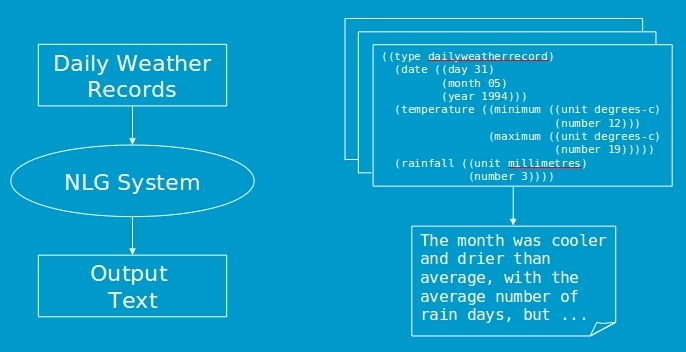
\includegraphics[scale=.3]{pics/pic6.jpg}
\end{center}

\end{frame}

\begin{frame}
\frametitle{The Architectural View}

\begin{center}
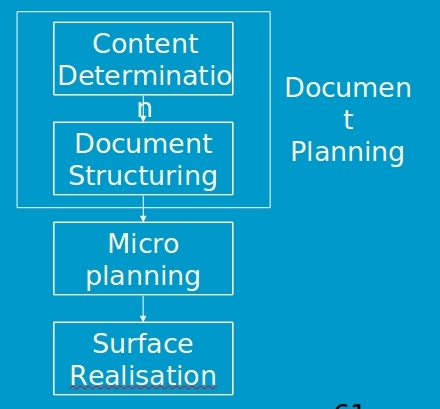
\includegraphics[scale=.3]{pics/pic7.jpg}
\end{center}
 
\end{frame}

\begin{frame}
\frametitle{Document Planning}

\label{f122}
\begin{itemize}
\item { {Goals: }}
\item { {to determine what information to communicate}}
\item { {to determine how to structure this information to make a coherent text}}
\item { {Two Common Approaches:}}
\item { {methods based on observations about common text structures}}
\item { {methods based on reasoning about discourse coherence and the purpose of the text }}
\end{itemize}

 
\end{frame}

\begin{frame}
\frametitle{Content Determination}

\label{f124}
\begin{itemize}
\item { {Based on MESSAGES, predefined data structures which:}}
\item { {correspond to informational elements in the text}}
\item { {collect together underlying data in ways that are convenient for linguistic expression}}
\item { {Core idea:}}
\item { {from corpus analysis, identify the largest possible agglomerations of informational elements that do not pre-empt required flexibility in linguistic expression}}
\end{itemize}

 
\end{frame}

\begin{frame}
\frametitle{Content Determination in WeatherReporter}

\label{f126}
\begin{itemize}
\item { {Routine messages}}
\begin{itemize}
\item MonthlyRainFallMsg, 
MonthlyTemperatureMsg, 
RainSoFarMsg, 
MonthlyRainyDaysMsg
\end{itemize}
\item { {Always constructed for any summary to be generated}}
\end{itemize}

 
\end{frame}

\begin{frame}
\frametitle{Content Determination in WeatherReporter}

\label{f128}
\begin{itemize}
\item { {A MonthlyRainfallMsg:}}
\begin{itemize}
\item 
{((message-id msg091)
 (message-type monthlyrainfall)
 (period ((month 04)
 (year 1996)))
 (absolute-or-relative relative-to-average)
 (relative-difference ((magnitude ((unit millimeters)
   (number 4)))
  (direction +))))}
\end{itemize}
\end{itemize}


\end{frame}

\begin{frame}
\frametitle{Content Determination in WeatherReporter}

\label{f130}
\begin{itemize}
\item { {Significant Event messages}}
\begin{itemize}
\item RainEventMsg, 
RainSpellMsg, 
TemperatureEventMsg, 
TemperatureSpellMsg
\end{itemize}
\item { {Only constructed if the data warrants their construction: eg if rain occurs on more than a specified number of days in a row}}
\end{itemize}

 
\end{frame}

\begin{frame}
\frametitle{Content Determination in WeatherReporter}

\label{f132}
\begin{itemize}
\item { {A RainSpellMsg:}}
\begin{itemize}
\item {
((message-id msg096)
 (message-type rainspellmsg)
 (period ((begin ((day 04)
  (month 02)
  (year 1995)))
 (end ((day 11)
 (month 02)
 (year 1995)))
 (duration ((unit day)
  (number 8)))))
 (amount ((unit millimetres)
 (number 120))))}
\end{itemize}
\item { {{}}}??
\end{itemize}

 
\end{frame}

\begin{frame}
\frametitle{Content Determination}

\label{f134}
\begin{itemize}
\item { {Alternative strategies:}}
\item { {Build all possible messages from the underlying data, then select for expression those appropriate to the context of generation}}
\item { {Identify information required for context of generation and construct appropriate messages from the underlying data}}
\end{itemize}

 
\end{frame}

\begin{frame}
\frametitle{Document Structuring via Schemas}

\label{f136}
\begin{itemize}
\item { {Basic idea (after McKeown 1985):}}
\item { {texts often follow conventionalised patterns}}
\item { {these patterns can be captured by means of \^atext grammars\^a that both dictate content and ensure coherent structure}}
\item { {the patterns specify how a particular document plan can be constructed using smaller schemas or atomic messages}}
\item { {can specify many degrees of variability and optionality}}
\end{itemize}

 
\end{frame}

\begin{frame}
\frametitle{Document Structuring via Schemas}

\label{f138}
\begin{itemize}
\item { {Implementing schemas:}}
\item { {simple schemas can be expressed as grammars}}
\item { {more flexible schemas usually implemented as macros or class libraries on top of a conventional programming language, where each schema is a procedure}}
\item { {currently the most popular document planning approach in applied NLG systems}}
\end{itemize}

 
\end{frame}

\begin{frame}
\frametitle{Deriving Schemas 
From a Corpus}

\label{f140}
\begin{itemize}
\item { {Using the Target Text Corpus:}}
\item { {take a small number of similar corpus texts}}
\item { {identify the messages, and try to determine how each message can be computed from the input data}}
\item { {propose rules or structures which explain why message \textit{x} is in text A but not in text B \^a this may be easier if messages are organised into a taxonomy}}
\item { {discuss this analysis with domain experts, and iterate}}
\item { {repeat the exercise with a larger set of corpus texts}}
\end{itemize}

\end{frame}

\begin{frame}
\frametitle{Document Planning in WeatherReporter}

\label{f142}
\begin{itemize}
\item { {A Simple Schema:}}

\item { {WeatherSummary \"{\i}{{\ooalign{\hfil\raise.07ex\hbox{R}\hfil\crcr\mathhexbox20D}}}}}
\begin{itemize}
\item MonthlyTempMsg
\item MonthlyRainfallMsg
\item RainyDaysMsg
\item RainSoFarMsg
\end{itemize}
\end{itemize}

 \end{frame}

\begin{frame}
\frametitle{Document Planning in WeatherReporter}

\label{f144}
\begin{itemize}
\item { {A More Complex Set of Schemata:}}

\item { {WeatherSummary \"{\i}{{\ooalign{\hfil\raise.07ex\hbox{R}\hfil\crcr\mathhexbox20D}}}}}
\begin{itemize}
\item TemperatureInformation RainfallInformation
\end{itemize}
\item { {TemperatureInformation \"{\i}{{\ooalign{\hfil\raise.07ex\hbox{R}\hfil\crcr\mathhexbox20D}}}}}
\begin{itemize}
\item MonthlyTempMsg \mbox{$[$}ExtremeTempInfo\mbox{$]$} \mbox{$[$}TempSpellsInfo\mbox{$]$}
\end{itemize}
\item { {RainfallInformation \"{\i}{{\ooalign{\hfil\raise.07ex\hbox{R}\hfil\crcr\mathhexbox20D}}}}}
\begin{itemize}
\item MonthlyRainfallMsg \mbox{$[$}RainyDaysInfo\mbox{$]$} \mbox{$[$}RainSpellsInfo\mbox{$]$}
\end{itemize}
\item { {RainyDaysInfo \"{\i}{{\ooalign{\hfil\raise.07ex\hbox{R}\hfil\crcr\mathhexbox20D}}}}}
\begin{itemize}
\item RainyDaysMsg \mbox{$[$}RainSoFarMsg\mbox{$]$}
\end{itemize}
\item { {...}}
\end{itemize}

\end{frame}

\begin{frame}
\frametitle{Schemas in Practice }

\label{f146}
\begin{itemize}
\item { {Tests and other machinery are often made explicit:}}

\item { {(put-template maxwert-grenzwert \"{}MV01\"{}}}
\item { { (:PRECOND (:CAT DECL-E}}
\item { { :TEST ((pred-eq 'maxwert-grenzwert)}}
\item { {  (not (status-eq (theme) 'no))))}}
\item { { :ACTIONS (:TEMPLATE (:RULE MAX-AVG-VALUE-E (self))}}
\item { {   \"{}. As a result, \"{}}}
\item { {  (:RULE EXCEEDS-THRESHHOLD-E (self))}}
\item { {   \"{}.\"{})))}}
\end{itemize}

 
\end{frame}

\begin{frame}
\frametitle{Schemas: Pros and Cons}

\label{f148}
\begin{itemize}
\item { {Advantages of schemas:}}
\item { {Computationally efficient}}
\item { {Allow arbitrary computation when necessary}}
\item { {Naturally support genre conventions}}
\item { {Relatively easy to acquire from a corpus}}
\item { {Disadvantages}}
\item { {Limited flexibility: require predetermination of possible structures}}
\item { {Limited portability: likely to be domain-specific}}
\end{itemize}
 
\end{frame}

\begin{frame}
\frametitle{Document Structuring via Explicit Reasoning}

\label{f150}
\begin{itemize}
\item { {Observation:}}
\item { {Texts are coherent by virtue of relationships that hold between their parts \^a relationships like narrative sequence, elaboration, justification ...}}
\item { {Resulting Approach:}}
\item { {segment knowledge of what makes a text coherent into separate rules }}
\item { {use these rules to dynamically compose texts from constituent elements by reasoning about the role of these elements in the overall text}}
\end{itemize}
 \end{frame}

\begin{frame}
\frametitle{Document Structuring via Explicit Reasoning}

\label{f152}
\begin{itemize}
\item { {Typically adopt AI planning techniques:}}
\begin{itemize}
\item Goal = desired communicative effect
\item Plan constituents = messages or structures that combine messages (subplans)
\end{itemize}
\item { {Can involve explicit reasoning about the user's beliefs}}
\end{itemize}
 
\end{frame}


\begin{frame}
\frametitle{Document Structuring in WeatherReporter}

\label{f178}
 
\end{frame}

\begin{frame}
\frametitle{More Complex Algorithms}

\label{f180}
\begin{itemize}
\item { {Adding complexity, following \mbox{$[$}Marcu 1997\mbox{$]$}:}}
\item { {Assume that multiple DocumentPlans can be created from a set of messages and relations}}
\item { {Assume that a desirability score can be assigned to each DocumentPlan}}
\item { {Determine the best DocumentPlan}}
\end{itemize}
 
\end{frame}

\begin{frame}
\frametitle{Document Planning}

\label{f182}
\begin{itemize}
\item { {Result is a DOCUMENT PLAN: a tree structure populated by messages at its leaf nodes}}
\item { {Next step: realising the messages as text}}
\end{itemize}
 
\end{frame}

\begin{frame}
\frametitle{Research Issues}

\label{f184}
\begin{itemize}
\item { {The use of expert system techniques in content determination -- for example, case based reasoning}}
\item { {Principled ways of integrating schemas and relation-based approaches to document structuring}}
\item { {A better understanding of rhetorical relations}}
\item { {Knowledge acquisition -- eg, methodologies for creating content rules, schemas, and relation applicability conditions for a particular application}}
\end{itemize}
 
\end{frame}

\begin{frame}
\frametitle{A Simple Realiser}

\label{f186}
\begin{itemize}
\item { {We can produce one output sentence per message in the document plan}}
\item { {A specialist fragment of code for each message type determines how that message type is realised}}
\end{itemize}
 
\end{frame}

\begin{frame}
\frametitle{The Document Plan}

\label{f188}
 
\end{frame}

\begin{frame}
\frametitle{A Simple Realiser}

\label{f190}
\begin{itemize}
\item { {For the MonthlyTemperatureMsg:}}
\item { {TempString = case (TEMP - AVERAGETEMP)}}
\begin{itemize}
\item \mbox{$[$}2.0 2.9\mbox{$]$}: \^a very much warmer than average.\^a
\item \mbox{$[$}1.0 1.9\mbox{$]$}: \^amuch warmer than average.\^a
\item \mbox{$[$}0.1 0.9\mbox{$]$}: \^aslightly warmer than average.\^a
\item \mbox{$[$}-0.1 -0.9\mbox{$]$}: \^aslightly cooler than average.\^a
\item \mbox{$[$}-1.0 -1.9\mbox{$]$}: \^amuch cooler than average.\^a
\item \mbox{$[$}-2.0 -2.9\mbox{$]$}: \^a very much cooler than average.\^a
\end{itemize}
\item { {endcase}}
\item { {Sentence = \^aThe month was\^a + TempString}}
\end{itemize}
 
\end{frame}

\begin{frame}
\frametitle{One Message per Sentence}

\label{f192}
\begin{itemize}
\item { {The Result:}}
\begin{itemize}
\item The month was cooler than average.
\item The month was drier than average.
\item There were the average number of rain days.
\item The total rain for the year so far is well below average. 
\item There was rain on every day for 8 days from 11th to 18th.
\item Rainfall amounts were mostly small.
\end{itemize}
\item { {The Target Text:}}
\begin{itemize}
\item The month was cooler and drier than average, with the average number of rain days, but the total rain for the year so far is well below average. 
Although there was rain on every day for 8 days from 11th to 18th, rainfall amounts were mostly small.
\end{itemize}
\end{itemize}
 
\end{frame}

\begin{frame}
\frametitle{Simple Templates}

\label{f194}
\begin{itemize}
\item { {Problems with simple templates in this example:}}
\item { {MonthlyTemp and MonthlyRainfall don\^at always appear in the same sentence}}
\item { {When they do appear in the same sentence, they don\^at always appear in the same order}}
\item { {Each can be realised in different ways: eg \^avery warm\^a vs \^awarmer than average\^a}}
\item { {Additional information may or may not be incorporated into the same sentence}}
\end{itemize}
 
\end{frame}

\begin{frame}
\frametitle{Microplanning}

\label{f196}
\begin{itemize}
\item { {Goal: }}
\item { {To convert a document plan into a sequence of sentence or phrase specifications}}
\item { {Tasks:}}
\item { {Paragraph and Sentence Aggregation}}
\item { {Lexicalisation}}
\item { {Reference}}
\end{itemize}
 
\end{frame}

\begin{frame}
\frametitle{The Architectural View}

\label{f198}
 
\end{frame}

\begin{frame}
\frametitle{Interactions in Microplanning}

\label{f200}
 
\end{frame}

\begin{frame}
\frametitle{Pipelined Microplanning}

\label{f202}
 
\end{frame}

\begin{frame}
\frametitle{Aggregation}

\label{f204}
\begin{itemize}
\item { {Combinations can be on the basis of}}
\item { {information content}}
\item { {possible forms of realisation}}
\item { {Some possibilities:}}
\item { {Simple conjunction}}
\item { {Ellipsis}}
\item { {Embedding}}
\item { {Set introduction}}
\end{itemize}
 
\end{frame}

\begin{frame}
\frametitle{Some Examples}

\label{f206}
\begin{itemize}
\item { {Without aggregation:}}
\begin{itemize}
\item Heavy rain fell on the 27th.
Heavy rain fell on the 28th.
\end{itemize}
\item { {With aggregation via simple conjunction:}}
\begin{itemize}
\item Heavy rain fell on the 27th and heavy rain fell on the 28th.
\end{itemize}
\item { {With aggregation via ellipsis: }}
\begin{itemize}
\item Heavy rain fell on the 27th and \mbox{$[$}\mbox{$]$} on the 28th.
\end{itemize}
\item { {With aggregation via set introduction: }}
\begin{itemize}
\item Heavy rain fell on \mbox{$[$}the 27th and 28th\mbox{$]$}.
\end{itemize}
\end{itemize}
 \end{frame}

\begin{frame}
\frametitle{An Example: Embedding}

\label{f208}
\begin{itemize}
\item { {Without aggregation:}}
\begin{itemize}
\item March had a rainfall of 120mm. 
It was the wettest month.
\end{itemize}
\item { {With aggregation:}}
\begin{itemize}
\item March, which was the wettest month, had a rainfall of 120mm.
\end{itemize}
\end{itemize}
 
\end{frame}

\begin{frame}
\frametitle{Choice Heuristics}

\label{f210}
\begin{itemize}
\item { {There are usually many ways to aggregate a given message set: how do we choose?}}
\item { {conform to genre conventions and rules}}
\item { {observe structural properties}}
\begin{itemize}
\item for example, only aggregate messages which are siblings in the document plan tree
\end{itemize}
\item { {take account of pragmatic goals}}
\end{itemize}
 
\end{frame}

\begin{frame}
\frametitle{Pragmatics: STOP Example}

\label{f212}
\begin{itemize}
\item { {Making the text friendlier by adding more empathy:}}
\begin{itemize}
\item It\^as clear from your answers that you don\^at feel too happy about being a smoker and it\^as excellent that you are going to try to stop.
\end{itemize}
\item { {Making the text easier for poor readers:}}
\begin{itemize}
\item It\^as clear from your answers that you don\^at feel too happy about being a smoker. It\^as excellent that you are going to try to stop.
\end{itemize}
\end{itemize}
 
\end{frame}

\begin{frame}
\frametitle{Aggregation in WeatherReporter}

\label{f214}
\begin{itemize}
\item { {Sensitive to rhetorical relations:}}
\item { {If two messages are in a SEQUENCE relation they can be conjoined at the same level}}
\item { {If one message is an ELABORATION of another it can either be conjoined at the same level or embedded as a minor clause or phrase}}
\item { {If one message is a CONTRAST to another it can be conjoined at the same level or embedded as a minor clause or phrase}}
\end{itemize}
 \end{frame}

\begin{frame}
\frametitle{An Aggregation Rule}

\label{f216}
 
\end{frame}

\begin{frame}
\frametitle{Lexicalisation}

\label{f218}
\begin{itemize}
\item { {The process of choosing words to communicate the information in messages}}
\item { {Methods:}}
\begin{itemize}
\item templates
\item decision trees
\item graph-rewriting algorithms
\end{itemize}
\end{itemize}
\end{frame}


\begin{frame}
\frametitle{
Lexical Choice}

\label{f0}
\begin{itemize}
\item {{If several lexicalisations are possible, consider:}}
\item {{user knowledge and preferences}}
\item {{consistency with previous usage}}
\begin{itemize}
\item in some cases, it may be best to vary lexemes
\end{itemize}
\item {{interaction with other aspects of microplanning}}
\item {{pragmatics}}
\begin{itemize}
\item It is encouraging that you have many reasons to stop.        (more precise meaning)
\item It\^as good that you have a lot of reasons to stop.                 (lower reading level)
\end{itemize}
\end{itemize}

\end{frame}

\begin{frame}
\frametitle{
WeatherReporter: Variations in Describing Rainfall}

\label{f3}
\begin{itemize}
\item {{Variations in syntactic category:}}
\item {{S:                \mbox{$[$}rainfall was very poor indeed\mbox{$]$}}}
\item {{NP:        \mbox{$[$}a much worse than average rainfall\mbox{$]$}}}
\item {{AP:        \mbox{$[$}much drier than average\mbox{$]$}}}
\item {{Variations in semantics:}}
\item {{Absolute:        \mbox{$[$}very dry\mbox{$]$}
                \mbox{$[$}a very poor rainfall\mbox{$]$}}}
\item {{Comparative:        \mbox{$[$}a much worse than average rainfall\mbox{$]$}
                \mbox{$[$}much drier than average\mbox{$]$} }}
\end{itemize}
\end{frame}

\begin{frame}
\frametitle{
WeatherReporter: 
Aggregation and Lexicalisation}

\label{f7}
\begin{itemize}
\item {{Many different results are possible:}}
\item {{The month was cooler and drier than average.
There were the average number of rain days, but the total rain for the year so far is well below average. There was rain on every day for 8 days from 11th to 18th, but rainfall amounts were mostly small.}}
\item {{The month was cooler and drier than average.
Although the total rain for the year so far is well below average, there were the average number of rain days.  There was a small mount of rain on every day for 8 days from 11th to 18th.}}
\end{itemize}
\end{frame}

\begin{frame}
\frametitle{
Referring Expression Generation}

\label{f9}
\begin{itemize}
\item {{How do we identify specific domain objects and entities?}}
\item {{Two issues:}}
\item {{Initial introduction of an object}}
\item {{Subsequent references to an already salient object}}
\end{itemize}
\end{frame}

\begin{frame}
\frametitle{
Initial Reference}

\label{f11}
\begin{itemize}
\item {{Introducing an object into the discourse:}}
\item {{use a full name}}
\begin{itemize}
\item Jeremy
\end{itemize}
\item {{relate to an object that is already salient}}
\begin{itemize}
\item Jane's goldfish
\end{itemize}
\item {{specify physical location}}
\begin{itemize}
\item the goldfish in the bowl on the table
\end{itemize}
\item {{Poorly understood; more research is needed}}
\end{itemize}
\end{frame}

\begin{frame}
\frametitle{
Subsequent Reference}

\label{f13}
\begin{itemize}
\item {{Some possibilities:}}
\item {{Pronouns}}
\begin{itemize}
\item \underbar{It} swims in circles.
\end{itemize}
\item {{Definite NPs}}
\begin{itemize}
\item \underbar{The goldfish} swims in circles.
\end{itemize}
\item {{Proper names, possibly abbreviated}}
\begin{itemize}
\item \underbar{Jeremy} swims in circles.
\end{itemize}
\end{itemize}
\end{frame}

\begin{frame}
\frametitle{
Choosing a Form of Reference}

\label{f15}
\begin{itemize}
\item {{Some suggestions from the literature:}}
\item {{use a pronoun if it refers to an entity mentioned in the previous clause, and there is no other entity in the previous clause that the pronoun could refer to}}
\item {{otherwise use a name, if a short one exists}}
\item {{otherwise use a definite NP}}
\item {{Also important to conform to genre conventions -- for example, there are more pronouns in newspaper articles than in technical manuals}}
\end{itemize}
\end{frame}

\begin{frame}
\frametitle{
Example}

\label{f17}
\begin{itemize}
\item {{I am taking the Caledonian Express tomorrow.  \underbar{It} is a much better train than the Grampian Express.  \underbar{The Caledonian} has a real restaurant car, while \underbar{the Grampian }just has a snack bar.   \underbar{The restaurant car} serves wonderful fish, while \underbar{the snack bar} serves microwaved mush.}}
\end{itemize}
\end{frame}

\begin{frame}
\frametitle{
Referring Expression Generation in WeatherReporter}

\label{f19}
\begin{itemize}
\item {{Referring to months:}}
\begin{itemize}
\item June 1999
\item June
\item the month
\item next June
\end{itemize}
\item {{Relatively simple, so can be hardcoded in document planning}}
\end{itemize}
\end{frame}

\begin{frame}
\frametitle{
Research Issues}

\label{f21}
\begin{itemize}
\item {{How do we make microplanning choices?}}
\item {{How do we perform higher-level aggregation, such as forming paragraphs from sentences?}}
\item {{How do we lexicalise if domain concepts do not straightforwardly map into words?}}
\item {{What is the best way of making an initial reference to an object?}}
\end{itemize}
\end{frame}

\begin{frame}
\frametitle{
Realisation}

\label{f23}
\begin{itemize}
\item {{Goal: }}
\begin{itemize}
\item to convert text specifications into actual text
\end{itemize}
\item {{Purpose: }}
\begin{itemize}
\item to hide the peculiarities of English (or whatever the target language is) from the rest of the NLG system
\end{itemize}
\end{itemize}
\end{frame}

\begin{frame}
\frametitle{
Realisation Tasks}

\label{f25}
\begin{itemize}
\item {{Structure Realisation:}}
\item {{Choose markup to convey document structure }}
\item {{Linguistic Realisation:}}
\item {{Insert function words}}
\item {{Choose correct inflection of content words}}
\item {{Order words within a sentence}}
\item {{Apply orthographic rules}}
\end{itemize}
\end{frame}

\begin{frame}
\frametitle{
Structure Realisation}

\label{f27}
\begin{itemize}
\item {{Add document markup}}
\item {{An example: means of marking paragraphs:}}
\begin{itemize}
\item HTML                        \mbox{$<$}P\mbox{$>$}
\item LaTeX                         (blank line)
\item RTF                        \mbox{$\backslash$}par
\item SABLE (speech)        \mbox{$<$}BREAK\mbox{$>$}
\end{itemize}
\item {{Depends on the document presentation system}}
\item {{Usually done with simple mapping rules}}
\end{itemize}
\end{frame}

\begin{frame}
\frametitle{
Linguistic Realisation}

\label{f29}
\begin{itemize}
\item {{Techniques:}}
\item {{Bi-directional Grammar Specifications}}
\item {{Grammar Specifications tuned for Generation}}
\item {{Template-based Mechanisms}}
\end{itemize}
\end{frame}

\begin{frame}
\frametitle{
Bi-directional Grammar Specifications}

\label{f31}
\begin{itemize}
\item {{Key idea:  one grammar specification used for both realisation and parsing}}
\item {{Can be expressed as a set of declarative mappings between semantic and syntactic structures}}
\item {{Different processes applied for generation and analysis}}
\item {{Theoretically elegant}}
\item {{To date, sometimes used in machine-translation systems, but almost never used in other applied NLG systems}}
\end{itemize}
\end{frame}

\begin{frame}
\frametitle{
Problems with the 
Bi-directional Approach}

\label{f33}
\begin{itemize}
\item {{Output of an NLU parser (a semantic form) is very different from the input to an NLG realiser (a text specification)}}
\item {{Debatable whether lexicalisation should be integrated with realisation}}
\item {{Difficult in practice to engineer large bidirectional grammars}}
\item {{Difficulties handling fixed phrases}}
\end{itemize}

\end{frame}

\begin{frame}
\frametitle{
Grammar Specifications tuned for Generation}

\label{f35}
\begin{itemize}
\item {{Grammar provides a set of choices for realisation}}
\item {{Choices are made on the basis of the input text specification}}
\item {{Grammar can \textit{only} be used for NLG}}
\item {{Working software is available}}
\begin{itemize}
\item Bateman's KPML
\item Elhadad's FUF/SURGE
\item CoGenTex\^as RealPro
\end{itemize}
\end{itemize}
\end{frame}

\begin{frame}
\frametitle{
Example: KPML}

\label{f37}
\begin{itemize}
\item {{Linguistic realiser based on Systemic Functional Grammar}}
\item {{Successor to Penman}}
\item {{Uses the Nigel grammar of English}}
\item {{Smaller grammars for several other languages available}}
\item {{Incorporates a grammar development environment}}
\end{itemize}
 
\end{frame}

\begin{frame}
\frametitle{
Systemic Grammar}

\label{f39}
\begin{itemize}
\item {{Emphasises the functional organisation of language}}
\item {{surface forms are viewed as the consequences of selecting a set of abstract functional features}}
\item {{choices correspond to minimal grammatical alternatives}}
\item {{the interpolation of an intermediate abstract representation allows the specification of the text to accumulate gradually}}
\end{itemize}
 
\end{frame}

\begin{frame}
\frametitle{
A Systemic Network}

\label{f41}
 
\end{frame}

\begin{frame}
\frametitle{
KPML}

\label{f43}
\begin{itemize}
\item {{How it works:}}
\item {{choices are made using INQUIRY SEMANTICS}}
\item {{for each choice system in the grammar, a set of predicates known as CHOOSERS are defined}}
\item {{these tests are functions from the internal state of the realiser and host generation system to one of the features in the system the chooser is associated with}}
\end{itemize}
 
\end{frame}

\begin{frame}
\frametitle{
KPML}

\label{f45}
\begin{itemize}
\item {{Realisation Statements:}}
\item {{small grammatical constraints at each choice point build up to a grammatical specification}}
\item {{\"{\i}!`Insert SUBJECT\"{\i}\mbox{$\pm$}:  an element functioning as subject will be present}}
\item {{\"{\i}!`Conflate SUBJECT ACTOR\"{\i}\mbox{$\pm$}:  the constituent functioning as SUBJECT is the same as the constituent that functions as ACTOR}}
\item {{\"{\i}!`Order FINITE SUBJECT\"{\i}\mbox{$\pm$}:  FINITE must immediately precede SUBJECT}}
\end{itemize}
 
\end{frame}

\begin{frame}
\frametitle{
Realisation Statements}

\label{f47}
 
\end{frame}

\begin{frame}
\frametitle{
An SPL input to KPML}

\label{f49}
\begin{itemize}
\item {{\textbf{(l / greater-than-comparison}}}
\item {{\textbf{  :tense past}}}
\item {{\textbf{  :exceed-q (l  a) exceed}}}
\item {{\textbf{  :command-offer-q notcommandoffer}}}
\item {{\textbf{  :proposal-q notproposal}}}
\item {{\textbf{  :domain (m / one-or-two-d-time :lex month :determiner the)}}}
\item {{\textbf{  :standard (a / quality :lex average determiner zero)}}}
\item {{\textbf{  :range (c / sense-and-measure-quality :lex cool)}}}
\item {{\textbf{  :inclusive (r / one-or-two-d-time}}}
\item {{\textbf{    :lex day}}}
\item {{\textbf{    :number plural}}}
\item {{\textbf{    :property-ascription (r / quality :lex rain)}}}
\item {{\textbf{    :size-property-ascription 
                         (av / scalable-quality :lex the-av-no-of)))}}}
\item {{\textbf{}}}??
\item {{\textbf{The month was cooler than average with the average number of rain days. }}}
\item {{\textbf{}}}??
\end{itemize}
 
\end{frame}

\begin{frame}
\frametitle{
Observation}

\label{f51}
\begin{itemize}
\item {{These approaches are geared towards broad-coverage linguistically sophisticated treatments}}
\item {{Most current applications don't require this sophistication:  much of what is needed can be achieved by templates or even canned text}}
\item {{But many applications will need deeper treatments for some aspects of the language}}
\item {{Solution:  integrate canned text, templates and \"{}realisation from first principles\"{} in one system}}
\end{itemize}
 
\end{frame}

\begin{frame}
\frametitle{
Busemann's TG/2}

\label{f53}
\begin{itemize}
\item {{Integrates canned text, templates and context free rules}}
\item {{All expressed as production rules whose actions are determined by conditions met by the input structure}}
\item {{Input structures specified in GIL, the Generation Interface Language; allows a portable interface}}
\item {{Output can easily include formatting elements}}
\end{itemize}
 
\end{frame}

\begin{frame}
\frametitle{
TG/2 Overview}

\label{f55}
 
\end{frame}

\begin{frame}
\frametitle{
A GIL Input Structure}

\label{f57}
\begin{itemize}
\item {{\mbox{$[$}(COOP wertueberschreitung)
           (TIME \mbox{$[$}(PRED dofc)
                  (NAME \mbox{$[$}(DAY 31) 
                         (MONTH 12) 
                         (YEAR 1996)\mbox{$]$})\mbox{$]$})
           (POLLUTANT so2)
           (SITE \"{}V\~A{\P}lklingen-City\"{})
           (THRESHOLD-VALUE \mbox{$[$}(AMOUNT 1000) 
                             (UNIT mkg-m3)\mbox{$]$})
           (DURATION \mbox{$[$}(DAY 30)\mbox{$]$})
           (SOURCE \mbox{$[$}(LAW-NAME vdi-richtlinie-2310)
                    (THRESHOLD-TYPE mikwert)\mbox{$]$})
           (EXCEEDS \mbox{$[$}(STATUS yes) 
                     (TIMES 4)\mbox{$]$})\mbox{$]$}}}
\end{itemize}
 
\end{frame}

\begin{frame}
\frametitle{
A TGL Rule}

\label{f59}
\begin{itemize}
\item {{(defproduction threshold-exceeding \"{}WU01\"{}
  (:PRECOND (:CAT DECL
             :TEST ((coop-eq 'threshold-exceeding)
                    (threshold-value-p)))
   :ACTIONS (:TEMPLATE
               (:OPTRULE PPTime (get-param 'time)
               (:OPTRULE SITEV (get-param site) 
               (:RULE THTYPE (self) 
               (:OPTRULE POLL (get-param 'pollutant) 
               (:OPTRULE DUR (get-param 'duration)
               \"{}(\"{} (:RULE VAL (get-param 'threshold-value)) 
                   (:OPTRULE LAW (get-param 'law-name)) \"{})\"{}
               (:RULE EXCEEDS (get-param 'exceeds)) \"{}.\"{}
             :CONSTRAINTS (:GENDER (THTYPE EXCEEDS) :EQ))))}}
\end{itemize}
 
\end{frame}

\begin{frame}
\frametitle{
TG/2 Output}

\label{f61}
\begin{itemize}
\item {{On 31-12-1996 at the measurement station at V\~A{\P}lklingen-City, the MIK value (MIK-Wert) for sulphur dioxide over a period of 30 days (1000 \^A\mbox{$\mu$}g/m\^A\mbox{${}^3$} according to directive VDI 2310 (VDI-Richtlinie 2310)) was exceeded four times. }}
\end{itemize}
 
\end{frame}

\begin{frame}
\frametitle{
Pros and Cons}

\label{f63}
\begin{itemize}
\item {{No free lunch:  every existing tool requires a steep learning curve}}
\item {{Approaches like TG/2 may be sufficient for most applications}}
\item {{Linguistically-motivated approaches require some theoretical commitment and understanding, but promise broader coverage and consistency}}
\end{itemize}
 
\end{frame}

\begin{frame}
\frametitle{
Morphology and Orthography}

\label{f65}
\begin{itemize}
\item {{Realiser must be able to:}}
\item {{inflect words}}
\item {{apply standard orthographic spelling changes}}
\item {{add punctuation}}
\item {{add standard punctuation rules}}
\end{itemize}
 
\end{frame}

\begin{frame}
\frametitle{
Research Issues}

\label{f67}
\begin{itemize}
\item {{How can different techniques (and linguistic formalisms) be combined?}}
\item {{What are the costs and benefits of using templates instead of \^adeep\^a realisation techniques? }}
\item {{How do layout issues affect realisation?}}
\end{itemize}
 
\end{frame}

\begin{frame}
\frametitle{
Overview}

\label{f69}
\begin{itemize}
\item {{1                An Introduction to NLG}}
\item {{2                Requirements Analysis and a Case Study}}
\item {{3                The Component Tasks in NLG}}
\item {{4                NLG in Multimedia and Multimodal Systems}}
\item {{5                Conclusions and Pointers}}
\end{itemize}
 
\end{frame}

\begin{frame}
\frametitle{
Document Types}

\label{f71}
\begin{itemize}
\item {{Simple ASCII (eg email messages)}}
\begin{itemize}
\item relatively straightforward: just words and punctuation symbols
\end{itemize}
\item {{Printed documents (eg newspapers, technical documents)}}
\begin{itemize}
\item need to consider typography, graphics
\end{itemize}
\item {{Online documents (eg Web pages)}}
\begin{itemize}
\item need to consider hypertext links
\end{itemize}
\item {{Speech (eg radio broadcasts, information by telephone)}}
\begin{itemize}
\item need to consider prosody
\end{itemize}
\item {{Visual presentation (eg TV broadcasts, MS Agent)}}
\begin{itemize}
\item need to consider animation, facial expressions
\end{itemize}
\end{itemize}
 
\end{frame}

\begin{frame}
\frametitle{
Typography}

\label{f73}
\begin{itemize}
\item {{Character attributes (italics, boldface, colour, font)}}
\begin{itemize}
\item can be used to indicate emphasis or other aspects of use:  typographic distinctions carry meaning
\end{itemize}
\item {{Layout (itemised lists, section and chapter headings)}}
\begin{itemize}
\item allows indication of structure, can enable information access
\end{itemize}
\item {{Special constructs provide sophisticated resources}}
\begin{itemize}
\item boxed text, margin notes, ...
\end{itemize}
\end{itemize}
 
\end{frame}

\begin{frame}
\frametitle{
Typographically-flat Text}

\label{f75}
\begin{itemize}
\item {{When time is limited, travel by limousine, unless cost is also limited, in which case go by train.  When only cost is limited a bicycle should be used for journeys of less than 10 kilometers, and a bus for longer journeys.  Taxis are recommended when there are no constraints on time or cost, unless the distance to be travelled exceeds 10 kilometers.  For journeys longer than 10  kilometers, when time and cost are not important, journeys should be made by hire car.}}
\end{itemize}
 
\end{frame}

\begin{frame}
\frametitle{
Structured Text}

\label{f77}
\begin{itemize}
\item {{\textit{When only time is limited}:}}
\begin{itemize}
\item travel by Limousine
\end{itemize}
\item {{\textit{When only cost is limited}:}}
\begin{itemize}
\item travel by Bus if journey more than10 kilometers
\item travel by Bicycle if journey less than10 kilometers
\end{itemize}
\item {{\textit{When both time and cost are limited}:}}
\begin{itemize}
\item travel by Train
\end{itemize}
\item {{\textit{When time and cost are not limited}:}}
\begin{itemize}
\item travel by Hire Car if journey more than10 kilometers
\item travel by Taxi if journey less than10 kilometers
\end{itemize}
\end{itemize}
 
\end{frame}

\begin{frame}
\frametitle{
Tabular Presentation}

\label{f79}
 
\end{frame}

\begin{frame}
\frametitle{
Diagrammatic Presentation}

\label{f81}
 
\end{frame}

\begin{frame}
\frametitle{
Text and Graphics}

\label{f83}
\begin{itemize}
\item {{Which is better?  Depends on:}}
\begin{itemize}
\item type of information communicated
\item expertise of user
\item delivery medium
\end{itemize}
\item {{Best approach: use both!}}
\end{itemize}
 
\end{frame}

\begin{frame}
\frametitle{
An Example from WIP}

\label{f85}
 
\end{frame}

\begin{frame}
\frametitle{
Similarities between
Text and Graphics}

\label{f87}
\begin{itemize}
\item {{Both contain sublanguages}}
\item {{Both permit conversational implicature}}
\item {{Structure is important in both}}
\item {{Both express discourse relations}}
\item {{Do we need a media-independent theory of communication?}}
\end{itemize}
 
\end{frame}

\begin{frame}
\frametitle{
Hypertext}

\label{f89}
\begin{itemize}
\item {{Generate Web pages!}}
\begin{itemize}
\item Dynamic hypertext
\end{itemize}
\item {{Models of hypertext}}
\begin{itemize}
\item browsing
\item question-space
\item dialogue
\end{itemize}
\item {{Model-dependent issues}}
\begin{itemize}
\item click on a link twice: same result both times?
\item discourse models for hypertext
\end{itemize}
\end{itemize}
 
\end{frame}

\begin{frame}
\frametitle{
Example:  Peba}

\label{f91}
 
\end{frame}

\begin{frame}
\frametitle{
Speech Output}

\label{f93}
\begin{itemize}
\item {{The NLG Perspective: enhances output possibilities}}
\begin{itemize}
\item communicate via spoken channels (eg, telephone)
\item add information (eg emotion, importance)
\end{itemize}
\item {{The speech synthesis perspective: intonation carries information}}
\begin{itemize}
\item Need information about syntactic structure, information status, homographs
\item Currently obtained by text analysis
\item Could by obtained from an NLG system automatically:  the idea of concept-to-speech
\end{itemize}
\end{itemize}
 
\end{frame}

\begin{frame}
\frametitle{
Examples}

\label{f95}
\begin{itemize}
\item {{\textit{John took a bow}}}
\begin{itemize}
\item Difficult to determine which sense of \textit{bow} is meant, and therefore how to pronounce it, from text analysis
\item But an NLG system knows this
\end{itemize}
\item {{\textit{John washed the dog}}}
\begin{itemize}
\item Should stress that part of the information that is new
\item An NLG system will know what this is
\end{itemize}
\end{itemize}
 
\end{frame}

\begin{frame}
\frametitle{
Overview}

\label{f97}
\begin{itemize}
\item {{1                An Introduction to NLG}}
\item {{2                Requirements Analysis and a Case Study}}
\item {{3                The Component Tasks in NLG}}
\item {{4                NLG in Multimedia and Multimodal Systems}}
\item {{5                Conclusions and Pointers}}
\end{itemize}
 
\end{frame}

\begin{frame}
\frametitle{
Applied NLG in 1999}

\label{f99}
\begin{itemize}
\item {{Many NLG applications being investigated }}
\item {{Few actually fielded}}
\begin{itemize}
\item but at least there are some: in 1989 there were none
\end{itemize}
\item {{We are beginning to see reusable software, and specialist software houses}}
\item {{More emphasis on mixing simple and complex techniques}}
\item {{More emphasis on evaluation}}
\item {{We believe the future is bright}}
\end{itemize}
 
\end{frame}

\begin{frame}
\frametitle{
Resources: SIGGEN}

\label{f101}
\begin{itemize}
\item {{SIGGEN (ACL Special Interest Group for Generation)}}
\item {{Web site at  
http://www.dynamicmultimedia.com.au/siggen}}
\begin{itemize}
\item resources: software, papers, bibliographies
\item conference and workshop announcements
\item job announcements
\item discussions
\item NLG people and places
\end{itemize}
\end{itemize}
 
\end{frame}


\end{document}
